\chapter{Analyse}

Das Analysekapitel beginnt mit einer Vorstellung einiger unterschiedlicher populärer Feature-Detektoren bzw. Deskriptoren. Anhand dieses Überblicks wird dann entschieden, welche Detektoren / Deskriptoren verwendet werden. Ein Vergleich von Bildern anhand von Features ist nicht unmittelbar möglich. Die Feature-Vektoren weisen viele Komponenten auf, was eine effiziente Berechnung nicht möglich macht.
Anschließend werden Verfahren betrachtet, die die entstandenen Feature-Deskriptoren gruppieren bzw. komprimieren um anhand dieser Darstellung eine Klassifizierung zu ermöglichen .Im Folgenden Kapitel Machine Learning werden Algorithmen die sich für diesen Zweck eignen untersucht. Zunächst wird auf den Prozess des unüberwachten Lernens eingegangen, um so die Auswahl möglicher Modelle einzuengen. Daraufhin erfolgt eine Auswahl an zwei Modelle die im Weiteren dieser Arbeit im Fokus stehen und realisiert werden. 
Da, je nach gewünschtem Modell, zum Aufbauen desselben, Tausende bis Millionen von Features verarbeitet werden müssen, wird bei der Betrachtung der beiden Ansätze geprüft, wie eine Beschleunigung der Berechnung durch parallele Verarbeitung erzielt werden kann. Gerade bei großen Datenmengen und einer enormen Datenparallelität können Probleme durch GPUs um ein vielfaches schneller gelöst werden als durch CPUs. Da Nvidias CUDA an der Hochschule Hannover sowohl gelehrt als auch zu Forschungszwecken genutzt wird und sich die \todo{Architektur} auch international in Forschung und Wirtschaft etabliert hat \todo{[REF]}, soll diese als technische Basis dienen. 

\section{Feature Deskriptoren}
\label{extraction}

Feature Deskriptoren enthalten Informationen von charakteristischen Bereichen in Bildern. Dabei kodieren sie weitaus mehr als nur die geometrische Position von Pixeln: Es wird beispielsweise die Beleuchtung und teilweise affine Invarianz berücksichtigt. In der Literatur finden sich verschiedene Ansätze, die je nach Einsatzgebiet unterschiedliche Stärken besitzen. Auf diese Weise soll auch ein Gefühl für die unterschiedlichen Arten von Deskriptoren und den vielfältigen Möglichkeiten der Feature-Auswahl und Beschreibung vermittelt werden. Nachfolgend werden einige Feature Deskriptoren vorgestellt, die verbreitete Anwendung durch ihre praktischen Erfolge erzielt haben. Für die weitere Verarbeitung der Features ist es erstrebenswert, dass ihre Darstellung möglichst kompakt ist. Deskriptoren werden als Vektoren von Zahlen kodiert, die abhängig vom Verfahren Informationen über einen Pixel und seine Nachbarschaft oder auch ein ganzes Bild enthalten. Je größer die Anzahl der Einträge eines Vektors, desto größer wird der Speicherbedarf und Rechenaufwand. Neben einer kompakten Darstellung werden daher in der Praxis weitere Verfahren verwendet, um die Anzahl der Komponenten eines Vektors zu reduzieren. 

\subsection{Local Binary Patterns}

Der Local Binary Pattern (LBP) Deskriptor erzeugt aus einem Bild eine Reihe Bitstrings als Deskriptoren. Die Länge der Bitstrings hängt hier von der verwendeten Größe der Nachbarschaft eines Pixel ab. Original wurde eine $3 \times 3$ Nachbarschaft verwendet, was zu einer Länge von acht führt (nur die Nachbarschaft wird kodiert). Für jeden Pixel wird nun bestimmt ob seine Intensität kleiner oder größer im Vergleich zu einem Schwellwert ist. Abhängig vom Ergebnis wird eine 0 oder 1 kodiert. Im Fall der $3 \times 3$ Nachbarschaft ergibt dies $2^8$ mögliche verschiedene Bitstrings, sodass der resultierende Featurevektor 256 Komponenten aufweist. LBP wurden um Invarianz gegenüber Rotationen und die Verarbeitung von Farbbildern erweitert. Durch die Entwicklung dieser Methode wurden vor allem im Bereich der Gesichtserkennung wesentliche Fortschritte gemacht \cite{lbp2002}. \todo{Bild}

\subsection{Spatial Envelope}

Einen ganz anderen Ansatz haben Torralba und Olivia \cite{mts2001} verfolgt: Statt Objekte durch lokale Features zu beschreiben, werden globale Eigenschaften betrachtet. Das Bild wird in einem Raum mit wenig Dimensionen abgebildet, dem sogenannten \textit{Spatial Envelope}. Die Autoren nutzen hier wahrnehmbare Dimensionen wie Natürlichkeit und Offenheit um den Raum zu definieren. Eine hohe Natürlichkeit weist zum Beispiel auf das Bild einer Landschaft hin: Hier kommen in der Regel kaum gerade vertikale und horizontale Linien vor, im Gegensatz zu Bildern, die von Menschen angefertigt wurden.  Bilder die in einer semantischen Kategorie Ähnlichkeiten aufweisen, liegen dann nah beieinander. Dieses Modell hat sich vor allem bewährt um eine Umgebung bzw. Landschaft zu klassifizieren. \todo{Bild}

\subsection{Histogram of Oriented Gradients}

Der Histogram of Orientied Gradients (HOG) Deskriptor beschreibt die Features als Histogramm der Richtung der Gradienten eines Bildes. Da sich Gradienten eignen um Kanten in Bildern zu erkennen, wird so die Form der Objekte eines Bildes erkannt. \todo{Dalal und Triggs \cite{hog2005} nutzten diesen Verfahren} bereits 2005, mit großem Erfolg, um Menschen in Bilder zu erkennen. 
Um ein HOG zu generieren wird das Bild in gleich große Zellen eingeteilt, die eine Nachbarschaft von Pixeln umfassen. Über die Pixel jeder Zelle werden nun die lokalen Gradienten berechnet. Diese fließen proportional zu ihrer Stärke in den kumulierten Gradienten der Zelle ein. Dabei hat jede Zelle eine feste, vorgegebene Anzahl an Klassen für die Orientierungen der Gradienten. 
Dalal und Triggs nutzten in ihrer Originalarbeit als Fenster eine 64 $\times$ 128 Nachbarschaft von Pixeln, eine Zellgröße von 8 $\times$ 8 Pixeln und $2 \times 2$ Zellen pro Block. In Abbildung \ref{img:hog} ist links das Fenster dargestellt und rechts die entsprechenden Gradienten der Zellen. 

\begin{figure}
	\centering
	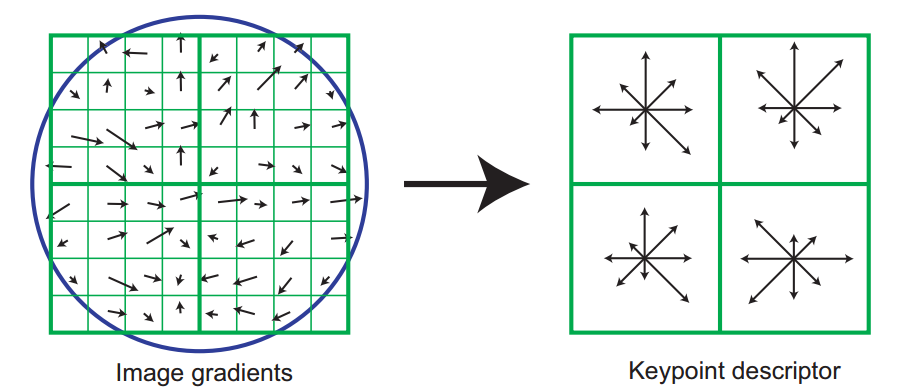
\includegraphics[scale=0.5]{images/hog.png}
	\caption{Schematische Darstellung des Histogram of Oriented Gradients  \cite{dif2004}}
	\label{img:hog}
\end{figure}

\subsection{SIFT}

SIFT ist ein Feature-Detektor und Deskriptor der 1999 von Lowe \cite{dif2004} entwickelt wurde. Neben der Invarianz der Skalierung der Features, berücksichtigt SIFT auch teilweise die Rotation, Beleuchtung und Perspektive. SIFT kombiniert mehrere mathematische Operationen und Verfahren um den Deskriptor eines Features als Ergebnis zu erhalten. Der Algorithmus lässt sich in vier wesentliche Schritte unterteilt:

\begin{enumerate}
	\item \textbf{Scale space} Im ersten Schritt wird die Invarianz der Skalierung behandelt. SIFT konstruiert hierfür einen \textit{scale space}. Hier werden aus dem Originalbild durch den \textit{Difference of Gaussians} immer verzerrtere Versionen erzeugt. Die Größe der neuen Bilder wird halbiert und die Prozedur wiederholt. Alle verzerrten Bilder einer Größe bilden eine sogenannte Oktave. SIFT verwendet vier Oktaven und fünf Bilder pro Oktave um den \textit{scale space} zu erzeugen. Um Ecken und Kanten in einem Bild zu ermitteln, die sich als Kandidaten für \textit{keypoints} eignen, wird nun zwischen allen aufeinanderfolgenden Bildern einer Oktave die Differenz gebildet. Das Prinzip ist für zwei Oktaven in Abbildung \ref{img:sift_dog} dargestellt. Das Ergebnis ist eine Approximation des Laplacian of Gaussians, jedoch ist dieses Verfahren weit weniger rechenintensiv. 

\begin{figure}
	\centering
	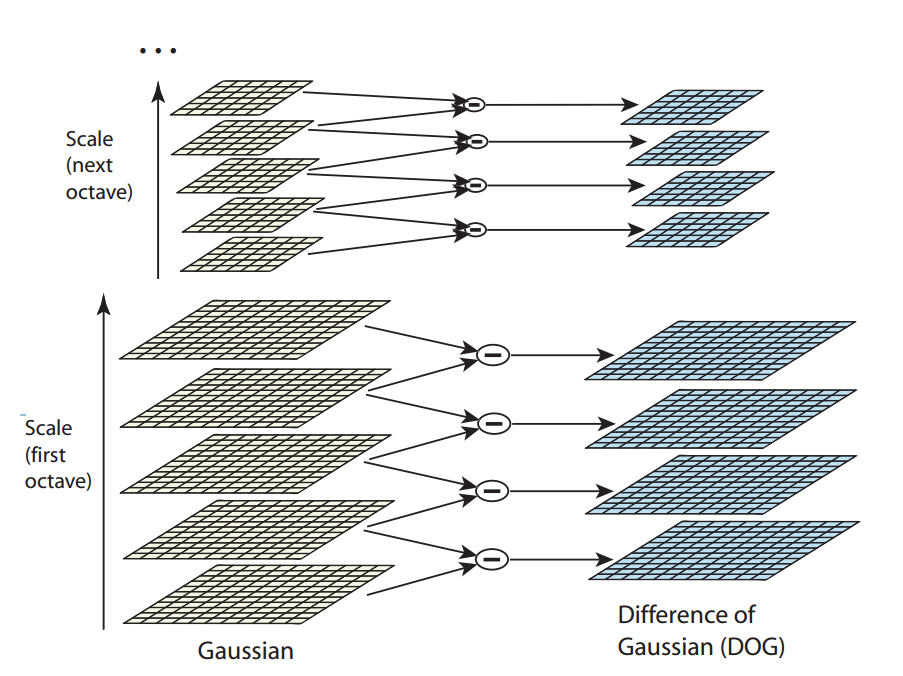
\includegraphics[scale=0.5]{images/sift_dog.png}
	\caption{Difference of Gaussians Operator \cite{dif2004}}
	\label{img:sift_dog}
\end{figure}	
	\item \textbf{Keypoint Ermittlung} Nicht alle Kandidaten werden zu \textit{keypoints}. Aus den DoG-Bildern werden nun die Extrempunkte bestimmt. Hierfür wird immer eine Nachbarschaft des DoG-Bildes und des vorigen und nachfolgendem im \textit{scale space} betrachtet. Da die Extremwerte nicht immer exakt auf einem Pixel liegen, muss die genau Position noch berechnet werden. SIFT verwendet hierfür eine Taylor Entwicklung im angenäherten \textit{keypoint} ausgehend.
	\item \textbf{Bestimmung der Orientierung} Bei dem Aufbau der Feature-Vektoren pro \textit{keypoint} wird die lokale Orientierung berechnet. Auf diese Weise sind die SIFT Deskriptoren invariant gegenüber Rotationen. Der SIFT Algorithmus berechnet ein Histogram of Oriented Gradients. Hierfür werden zufällig Punkte aus der Nachbarschaft des \textit{keypoints} ausgewählt. Der Extremwert des Histogramms wird dann als dominante Orientierung verwendet.
	\item \textbf{Deskriptor} Für jeden durch den Detektor gefundenen \textit{keypoint} wird nun ein Feature-Vektor gebildet. Der Feature-Vektor enthält Informationen über die Nachbarschaft in Form der Gradienten. Das Fenster für die Auswahl der Nachbarschaft wird auf dem \textit{keypoint} zentriert und in vier Teilfenster unterteilt. Die Gradienten in allen Teilfenster werden in acht Richtungen gemessen, sodass der resultierende Deskriptor 128 Komponenten enthält.
\end{enumerate}

SIFT ist äußerst robust, da Änderungen im Grenzwert von Position und Orientierung den Feature-Vektor kaum beeinflussen. Der Deskriptor besitzt zwar keine affine Invarianz, in praktischen Anwendungen werden jedoch auch mit skalierten, rotierten und verschobenen Objekten gute Ergebnisse erzielt. Mikolajczyk und Schmid haben 2005 SIFT mit anderen Deskriptoren wie \todo{DESC} verglichen und kamen zu dem Ergebnis, dass SIFT sehr gut hinsichtlich \todo{der Geschwindigkeit und des Speicherbedarfs} performt \cite{idp2005}. Die Konstruktion des Deskriptors ist allerdings sehr aufwendig und die Beschreibung erfordert einen Feature-Vektor mit 128 Komponenten.

\subsection{Bewertung der Deskriptoren}

Eine wesentliche Eigenschaft die der Deskriptor aufweisen sollte, ist affine Invarianz. Verschiedene Objekte oder Merkmale die auf mehreren Bildern vorhanden sind, besitzen selten die gleiche Position, daher sollten Rotation, Skalierung und Translationen berücksichtigt werden können. Gegenwärtig ist aber noch kein Deskriptor vorhanden, der eine Einbeziehung aller möglichen Umstände realisiert. In der Literatur und Praxis hebt sich von allen Deskriptoren der SIFT-Deskriptor in dieser Hinsicht am meisten ab. Zwar gibt es für spezielle Anwendungsfälle geeignetere Deskriptoren, wie beispielsweise den LBP-Deskriptor für die Erkennung von Passanten, doch SIFT ist bis heute der beste \glqq Allrounder\grqq  zur Objekterkennung. Insofern ist SIFT auch ein guter Ausgangspunkt, wenn mehr als eine spezielle Objektart berücksichtigt werden muss. Generell funktionieren die im folgenden vorgestellten Modelle mit jeder Art von (Bild-)Deskriptor: Die Modelle arbeiten genau aus diesem Grund nicht direkt mit den Bilddaten, sondern den Deskriptoren. Bei eben diesen handelt es sich lediglich um Vektoren aus dem Raum $\mathbb{R}^d$, wobei die Dimensionalität $d$ des Raums und damit die Anzahl der Elemente des Vektors abhängig vom Verfahren sind. Dies schränkt aber nicht die generelle Machbarkeit ein, sondern wirkt sich auf die Laufzeit bzw. den Speicherbedarf aus. Da für die vorliegenden Bilddaten der HsH keine speziellen Annahmen getroffen werden können, wird für die Gewinnung der \text{keypoints} das SIFT-Verfahren verwendet. 

\todo{Komponenten von SIFT betrachten, zwar viele aber nicht genug für alle Verfahren}
\todo{Eventuell ML anschließen, nach Modellwahl?}
\todo{Überleitung wie das in die Modelle passt, warum Gradienten für AE}

\section{Machine Learning}

Machine Learning ist ein Teilgebiet der künstlichen Intelligenz und wird genutzt um System zu entwerfen, die nicht explizit programmiert werden. Stattdessen Lernen diese Systeme: Lernen bedeutet in diesem Kontext, dass eine System durch eine Eingabe seine Struktur verändert, um so die erwartete Leistung zu steigern. Dabei ist Machine Learning ein interdisziplinäres Feld: Es sind sowohl Computerwissenschaften, Statistik als auch biologische und kognitive Wissenschaften involviert. Bisher haben sich viele Anwendungsfälle für Machine Learning Verfahren ergeben, die bis in den Alltag reichen. Einige Beispiele sind:

\begin{itemize}
	\item \textbf{Optical Character Recognition (OCR)} Unter OCR wird das Übersetzen eines (hand-)geschriebenen Textes in eine digitales Dokument bezeichnet. Beispielsweise kann so das Einfügen von Daten in CRM / ERP System automatisiert werden.
	\item \textbf{Spam Filterung} Das automatische Erkennen von unerwünschten E-Mails, die Werbung enthalten oder Betrugsversuche sind, ist inzwischen bei jedem Mail-Anbieter Teil des Angebots.
	\item \textbf{Spracherkennung} Auch eine Spracherkennung ist bereits auf den meisten digitalen Assistenten verfügbar und wird sogar zur Steuerung der häuslichen Elektronik verwendet.
	\item \textbf{Anomalie Erkennung} Digitale Geldtransaktionen werden heute von Algorithmen überwacht, die Abweichungen im Zahlungsverhalten beobachten. Wird eine ungewöhnlich hohe Summe überwiesen oder abgehoben, kann so informiert und auch interveniert werden.
\end{itemize}

All diese Verfahren Nutzen eine große Menge an Trainingsdaten, um so ein Modell zu generieren, welches eine Klassifizierung weiterer Daten ermöglicht. Beispielsweise müssen bei einem System zur Spam Filterung sowohl \glqq normale\grqq  als auch Spam E-Mails verwendet werden, eine Spracherkennung benötigt digitale Aufnahmen von Wörtern und Sätzen zum Lernen, etc.
Nach dem Aufbau des Modells findet dann durch das System die Klassifizierung von Test- bzw. realen Daten statt. Es wird beispielsweise bei OCR entschieden, welches digitale Pendant zum vorliegenden Zeichen gehört oder wie hoch die Wahrscheinlichkeit ist, dass es sich bei einer Mail um Spam handelt. Diese Trainings- und Testphase sind typisch für Machine Learning Verfahren. Allgemein eignet sich dieser Ansatz:

\begin{itemize}
	\item Um Beziehungen und Muster in den Daten zu entdecken, die nicht offensichtlich sind. Im Wesentlichen beschäftigt sich die Disziplin \textit{Data Mining} mit dieser Fragestellung und nutzt u.a. Machine Learning Verfahren.
	\item Wenn kein klassischer Algorithmus für die Problemstellung entworfen werden kann oder das Programm zu komplex ist, als das es von Menschen kodiert und gewartet werden könnte.
	\item Um neue Informationen einzubeziehen. Das Modell basiert auf den Daten, daher kann das System sich durch neue Daten verändern und so der Situation anpassen.
\end{itemize}

\subsection{Lernverfahren}

Je nach Fragestellung haben sich unterschiedliche Methodiken entwickelt, um den Lernprozess in einem System abzubilden. Im Wesentlichen werden drei Arten des maschinellen Lernens unterschieden:

\begin{itemize}
	\item \textbf{Überwachtes Lernen (supervised learning)} Ein überwachtes Lernverfahren soll eine Funktion lernen, die Eingaben ihren Ausgaben zuordnet. Diese Funktion wird anhand von Trainingsdaten gelernt, die demzufolge aus Paaren von Eingaben und ihren dazugehörigen Ausgaben bestehen.
	\item \textbf{Unüberwachtes Lernen (unsupervised learning)} Ziel unüberwachter Lernalgorithmen ist es, großen Mengen von nicht kategorisierten Daten zu gruppieren oder zu komprimieren. Dadurch können Beziehungen in den Daten entdeckt bzw. kompaktere Darstellungen erreicht werden.
	\item \textbf{Verstärkendes Lernen (reinforcement learning)} Beim verstärkenden Lernen hat ein Agent die Aufgabe ein vorgegebenes Ziel zu erreichen, indem er mit seiner Umwelt agiert. Die Umwelt ist dabei eine Menge von Zuständen zwischen denen der Agent durch eine Aktion wechselt. Dabei hat jede Aktion eine Belohnungen oder Bestrafungen zufolge. Der Agent optimiert dann sein Verhalten, um die erhaltenen Belohnungen zu maximieren.
\end{itemize}

Überwachte und unüberwachte Lernverfahren unterscheiden sich im Wesentlichen über ihre Annahmen in der kausalen Struktur: Beim überwachten Lernen ist es notwendig, dass sowohl Ursachen (Eingaben) als auch Effekte (Ausgaben) gemessen wurden. Beim unüberwachten Lernen hingegen sind die Eingaben latente Variablen. Das heißt sie sind nicht direkt gemessen worden, sondern durch mathematische Verfahren von Observationen abgeleitet. Dadurch ist ein exploratives Vorgehen möglich. Es können Beziehungen in den Daten entdeckt und Gruppierungen bzw. Klassifizierungen durchgeführt werden. \todo{Why unsupervised}

\subsection{Auswahl geeigneter Modelle}

Für die Featuregewinnung eignen sich vor allem unüberwachte Lernverfahren, \todo{warum} da pro Bild viele Deskriptoren gefundenen werden, die in einem hochdimensionalen Raum liegen. Zum einen muss die Menge der erzeugten Deskriptoren auf die Wesentlichen reduziert werden, zum anderen eignen sich die SIFT Feature-Vektoren mit ihren 128 Elementen nur bedingt für einen direkten Vergleich. \todo{Hier: denkbar größerer Feature-Vektor, den ein Netz lernt} Eine Möglichkeit besteht darin, durch ein Clustering Verfahren die Deskriptoren in Kategorien zu quantisieren, sodass beim \textit{Labeling} eines Bildes nur noch ein Bruchteil an Vergleichen durchgeführt werden muss. Ein anderer Ansatz ist das Verringern der Feature Dimensionalität. Verfahren wie beispielsweise die Hauptkomponentenanalyse bilden die Feature-Vektoren auf einen Raum niederer Dimensionen ab und wurden bereits speziell für SIFT adaptiert (SIFT-PCA). Für diesen Zweck wurden auch neuronale Netze adaptiert. \todo{Convolutional}. Ein Autoencoder hingegen ist ein spezielles neuronales Netzwerk, welches für das Lernen einer komprimierten Darstellung von Daten verwenden wird.

Aus den möglichen Modellen sollen der Bag of Visual Words und der Autoencoder umgesetzt werden. Der Bag of Visual Words führt im Wesentlichen ein Clustering der Feature-Vektoren durch und erreicht so eine kompakte Histogrammdarstellung dieser. K-means ist ein bekanntes und etabliertes Verfahren, dass inzwischen auch für die parallele Ausführung auf Grafikkarten adaptiert wurde.
\todo{NN}.
Im Folgenden werden zwei verschiedene unüberwachte Lernverfahren, dass Bag of Visual Words Modell und der Autoencoder, vorgestellt. Ziel ist es beide Verfahren zu implementieren und die Ergebnisse gegenüberzustellen.
\todo{TODO, BoVW (etabliert, kmeans, data mining) und AE (neu, ML, kompression)}

\section{Ansatz 1: Bag of Visual Words}

Im ersten Ansatz soll das Bag of Visual Words Modell genutzt werden. Zu Beginn liegen die Feature-Vektoren vor, die in der vorigen Phase extrahiert wurden. Um das Codebook aufzubauen ist es erforderlich, die \textit{Visual Words} zu generieren. Die \textit{Visual Words} werden durch ein Clustering der Feature-Vektoren gewonnen, daher handelt es sich hier um ein unüberwachtes Lernverfahren. Als Clustering Algorithmus wird hier Llyods heuristische Variante des k-means Algorithmus verwendet. Zunächst wird eine gängige sequentielle Implementierung angeführt, auf deren Basis dann die Parallelisierbarkeit durch Grafikkarten untersucht wird. Bei der Einordnung eines Bildes wird ein Histogramm der Visual Words generiert, daher wird im Anschluss ein sequentieller Histogramm Algorithmus vorgestellt, der auf Parallelisierbarkeit geprüft wird.

\subsection{Lloyds Algorithmus}

Im Grundlagenkapitel wurde bereits Lloyds Algorithmus eingeführt, hier soll zunächst näher auf die sequentielle Ausführung eingegangen werden, um anschließend eine mögliche Parallelisierung zu diskutieren. Im nachfolgenden Codelisting ist der Ablauf des Algorithmus in Pseudocode beschrieben. Als Parameter werden die Punkte $P$ und die Anzahl der zu bildenden Cluster $k$ erwartet. In Zeile 2 findet die Auswahl der initialen Schwerpunkte der Cluster statt. Die Zuordnung von Punkten zu Clustern erfolgt in Zeile 7: $argminD$ wählt den Cluster aus, dessen Varianz am wenigsten bei Aufnahme des Punktes $p_{i}$ steigt. Abschließend wird die Aktualisierung der Schwerpunkte aller Cluster in Zeile 9 durchgeführt.

\lstset{language=C}
\begin{lstlisting}[mathescape=true]
kmeans_lloyd ($P, C, k$)
	initialisierung
	until convergence
		$C_{j} = 0, j = 1, ..., k$
		for each $p_{i} \in P$
			for each $c_{j} \in C$
				$c_{j} = argminD(c_{j}, p_{i})$		
		for each $c_{j} \in  C$
			$c_{j} = \frac{1}{|c_{j}|} \sum_{n_{i} \in c_{j}} n_{i}$
\end{lstlisting}

Die Initialisierungsphase muss für die Parallelisierung nicht beachtet werden: Sie nimmt nur wenig Zeit in Anspruch und wird einmalig zu Beginn ausgeführt. Die anderen beiden Schritte des Algorithmus bergen mehr Potential: In Zeile 5 bis 7 wird die Varianz jedes Cluster-Vektor Paares berechnet. Da die Berechnung der Varianz eines Paares unabhängig von der eines anderen ist, kann die Berechnung aller Varianzen parallel erfolgen. Nachdem für einen Durchgang die Veränderung der Mitgliedschaft von Vektoren zu Clustern berechnet wurde, müssen die Cluster-Schwerpunkte aktualisiert werden. Auch die Berechnung der neuen Schwerpunkte der Cluster kann unabhängig voneinander erfolgen: Die Vektoren aus denen der Mittelwert berechnet wird, sind genau einem Cluster zugeordnet.

% http://www.know-center.tugraz.at/download\_extern/papers/latex8.pdf

\subsection{Histogramme}

Ein sequentielles Histogramm kann als Programm in einer Schleife über die Daten ausgedrückt werden: Für jedes Element wird der Index der Klasse des Histogramms berechnet und um eins inkrementiert. Zur Normalisierung des Histogramms ist es anschließend notwendig, jede Klasse des Histogramms durch die Gesamtanzahl der Werte zu dividieren. Da es sich bei der Anzahl der Klassen jedoch um eine kleine Zahl, im Vergleich zur Anzahl der Elemente in den Daten, handelt, ist dieser Aufwand vernachlässigbar.
Um das Histogramm der Visual Words eines Bildes zu erzeugen, muss für jedes extrahierte Feature das nächste Visual Word bestimmt werden. Dies entspricht im nachfolgenden Pseudocode der doppelten Schleife über die Features $F$ und Cluster $C$ in Zeile 2 und 3. Der Index des nächsten Clusters wird dann in Zeile 4 durch $argmin D$ berechnet und in der nächsten Zeile wird das Histogramm $H$ an der entsprechenden Stelle inkrementiert.

\begin{lstlisting}[mathescape=true]
histogram ($P, C, H$)
	for each $p_{i} \in P$
		for each $c_{j} \in C$
			$k = arminD(c_{j}, p_{i})$ 
		$H_{k} = H_{k} + 1$		
	for $1 .. |H|$
		$H_{i} = H_{i} / |H|$
\end{lstlisting}

\section{Ansatz 2: Autoencoder}

Durch den Aufschwung des maschinellen Lernens in den letzten Jahren sind neuronale Netze stark in den Fokus der Industrie und Wissenschaft gerückt. Solche künstlichen neuronalen Netze werden genutzt, um aus Beispielen Muster zu lernen und diesen Wissen zu transferieren. 
Ein spezielles neuronales Netzwerk zum unbeaufsichtigten Lernen ist der Autoencoder. Diese Art von Netzwerk lernt selbstständig eine komprimierte Darstellung der Eingabe. Eine Einführung in die Funktionsweise ist im Grundlagenkapitel unter dem Abschnitt REF[AE] zu finden.
\todo{Einleitung AE in Bildverarbeitung, Schwierigkeit Konstruktion AE, daher Zhao}. Ein Autoencoder der mit Feature-Deskriptoren von Bildern arbeitet, wurde von Zaho \cite{aed2016} vorgeschlagen. In einem Experiment wurde gezeigt, dass dieser Autoencoder \textit{state of the art} Ergebnisse erzielt: die Ergebnisse wurden unter verschiedenen Kriterien mit denen der Hauptkomponentenanalyse (PCA) und SIFT-PCA verglichen. Dabei erkannte der Autoencoder in fast allen die gleichen Features, jedoch durch einen 36 statt 128-elementigen Feature-Vektor. Aus diesem Grund soll Zhaos Autoencoder adaptiert werden. Der hierfür verwendete Feature Deskriptor und der Aufbau des Netzes werden im Kapitel \ref{AEFeatures} beschrieben.

\subsection{Autoencoder in der Bildverarbeitung}

\todo{Allgemeines}

\subsection{Autoencoder für Bild Features}
\label{AEFeatures}
Ein populäres Beispiel für die Verwendung von Autoencoder ist das Erkennen von Ziffern in einem Bild. Solch ein Netzwerk arbeitet direkt mit den Pixeln des Bildes: Bei einem Bild mit $m \times n$ Pixeln, umfasst die erste Schicht ebenfalls $m \times n$ Neuronen, für jeden Pixel Eines. Wie üblich, umfassen die folgenden Schichten weniger Neuronen. Durch eine abschließende Schicht zur Klassifizierung wird das Bild schließlich eingeordnet. Da aber in vielen Anwendungsfällen nicht direkt mit Pixeln gearbeitet werden kann, ist es wünschenswert, dass der Autoencoder stattdessen mit Features von Bildern arbeitet. Für die Extraktion geeigneter \textit{keypoints} hat sich der SIFT-Detektor bewährt, der Deskriptor hat jedoch bereits eine zu kompakte Darstellung um ein tiefes Netzwerk aufzubauen.
\todo{Viele Parameter und Entscheidungen, daher Zhaos Ansatz (Anzahl Layer, Anzahl Neuronen pro Schicht, Aktivierungsfunktionen , Art der Verbindungen (Pooling, etc), meist fully connected in Beispielen, Feature-Größe beeinflusst gesamte Netzarchitektur)}
Zhao \cite{aed2016} hat aus diesem Grund einen anderen Feature-Vektor erzeugt, der dann anschließend durch einen Autoencoder komprimiert wird. Dieser Feature-Vektor ist eine Kodierung der Gradienten von Patches in vertikale und horizontale Richtung. Die Patches sind hier eine Nachbarschaft der Größe $41 \times 41$, jeweils zentriert auf einem\textit{keypoint}. Letztendlich wird ein Feature-Vektor mit 3042 Elementen erzeugt, der durch den Autoencoder komprimiert werden soll.
Der Feature-Vektor mit 3042 Elementen bildet nun eine gute Basis, um einen mehrschichtigen Autoencoder zu entwickeln, der sukzessiv eine abstraktere Repräsentation lernt. Der von Zhao vorgeschlagene Encoder besteht aus fünf Stufen. Die erste Schicht besteht aus 3042 Neuronen um die Eingabe weiterzuleiten. Folgend werden 1024, 512, 128 und schließlich 36 Neuronen für die Kodierung verwendet. Der Decoder ist umgekehrt aufgebaut und auch die Gewichte der Kanten zwischen zwei Neuronen entsprechen ihren Pendants im Encoder.

\todo{Zhaos Grafik und Parameter aufführen, dann in Konzeption eigenes Modell}